\documentclass{standalone}
\usepackage{tikz}
\usetikzlibrary{patterns, positioning}
\usepackage[sfdefault]{ClearSans} %% option 'sfdefault' activates Clear Sans as the default text font
\usepackage[T1]{fontenc}

\begin{document}
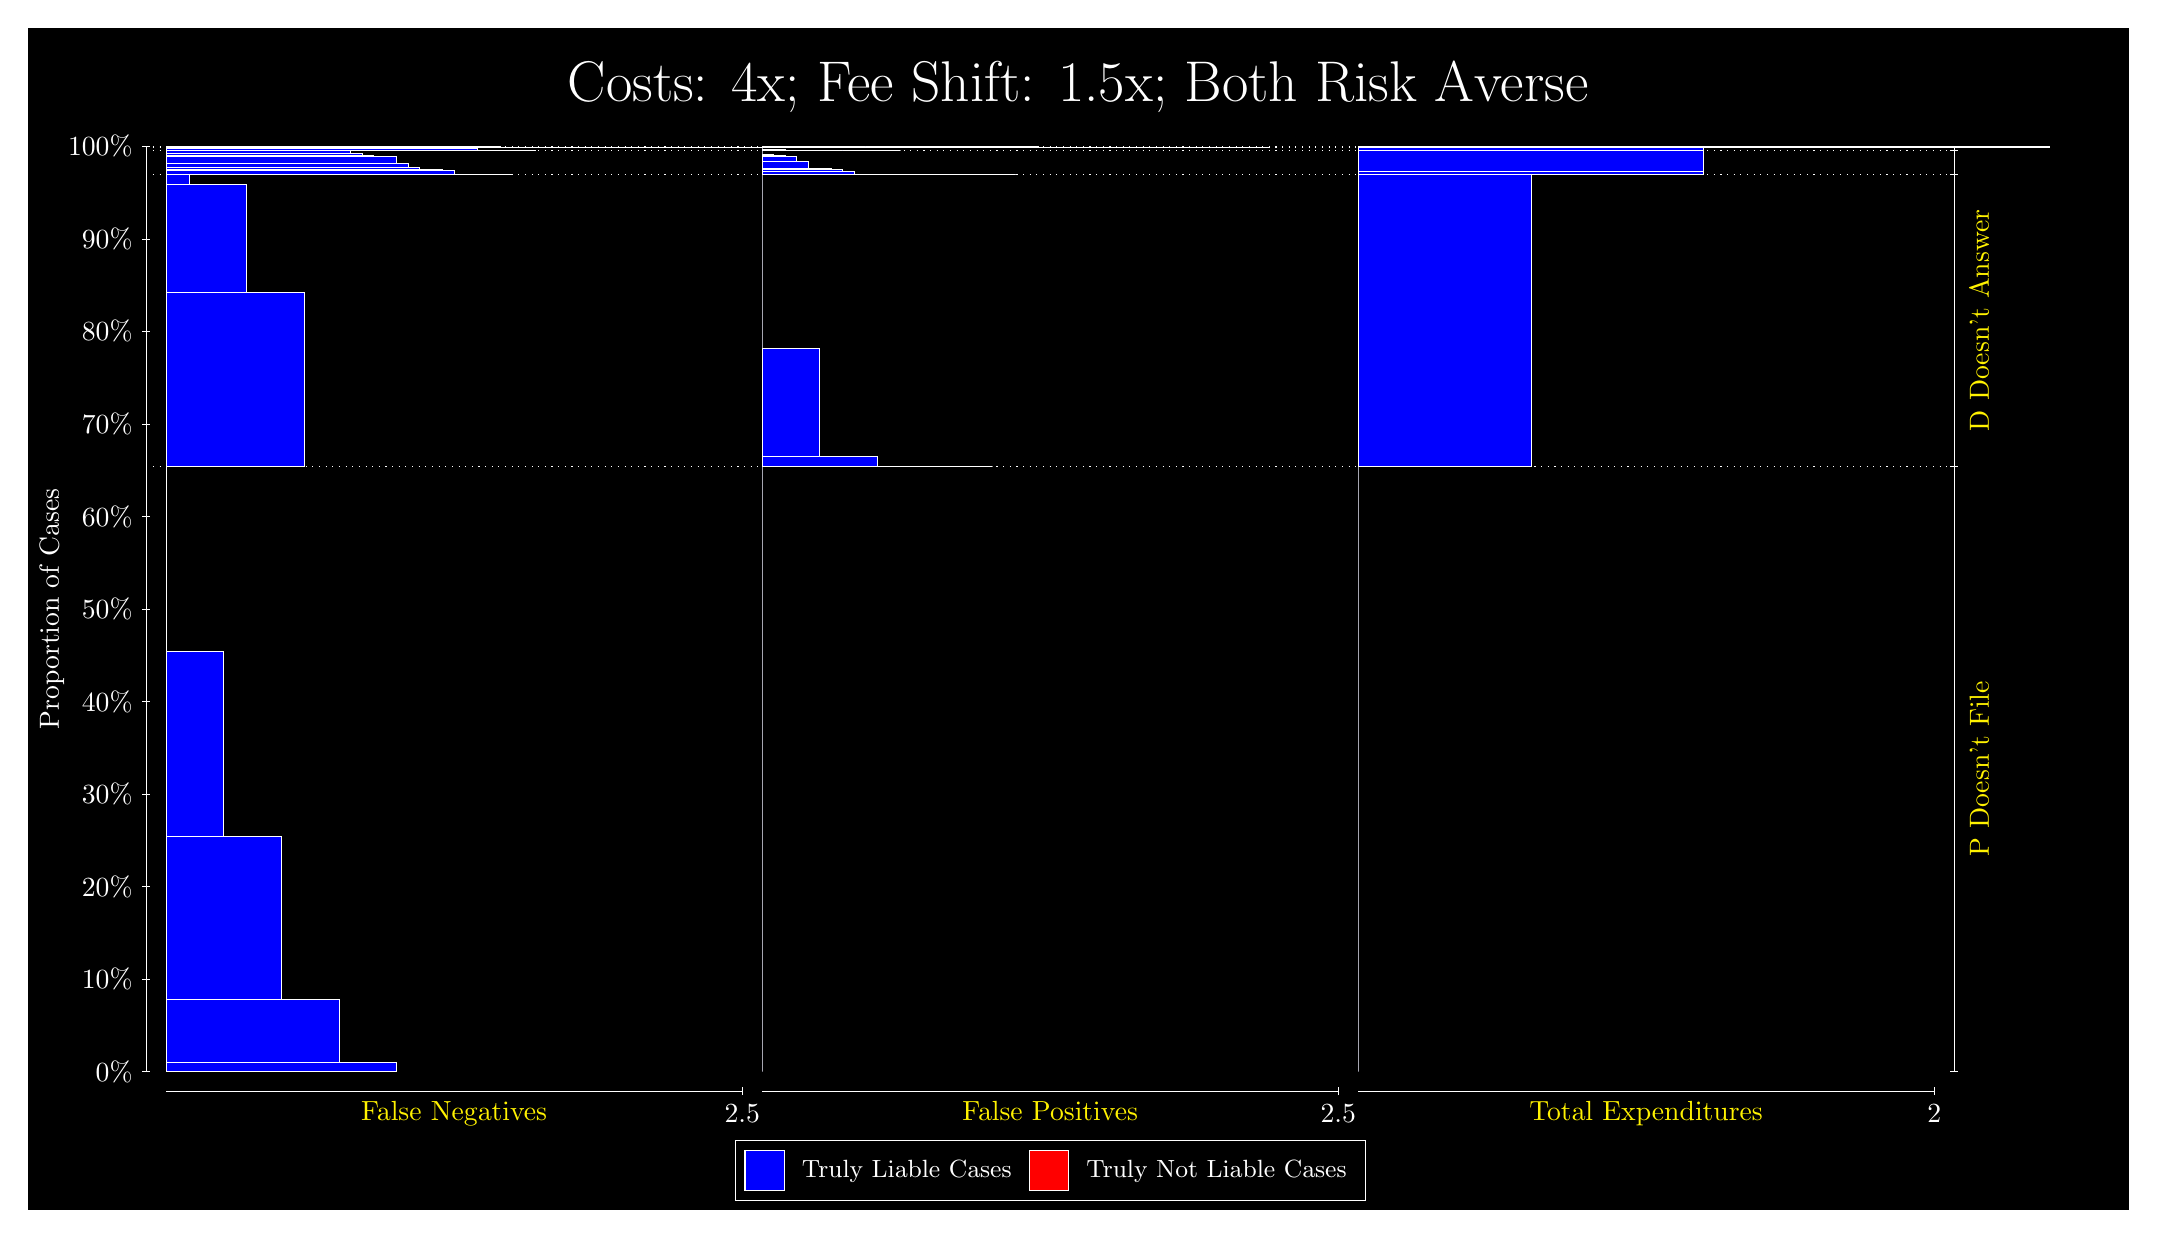
\begin{tikzpicture}
\draw[fill=black] (0,0) rectangle (26.667,15);
\draw[text=white] (0,13.5) rectangle (26.667,15) node[midway] {\huge Costs: 4x; Fee Shift: 1.5x; Both Risk Averse};
\draw[white, very thin] (1.5,1.75) -- (1.5,13.5);
\node[rotate=90, text=white, anchor=center] at (0.3, 7.625) {Proportion of Cases};
\draw[white, very thin] (1.45,1.75) -- (1.55,1.75);
\node[text=white, anchor=east] at (1.45, 1.75) {0\%};
\draw[white, very thin] (1.45,2.925) -- (1.55,2.925);
\node[text=white, anchor=east] at (1.45, 2.925) {10\%};
\draw[white, very thin] (1.45,4.1) -- (1.55,4.1);
\node[text=white, anchor=east] at (1.45, 4.1) {20\%};
\draw[white, very thin] (1.45,5.275) -- (1.55,5.275);
\node[text=white, anchor=east] at (1.45, 5.275) {30\%};
\draw[white, very thin] (1.45,6.45) -- (1.55,6.45);
\node[text=white, anchor=east] at (1.45, 6.45) {40\%};
\draw[white, very thin] (1.45,7.625) -- (1.55,7.625);
\node[text=white, anchor=east] at (1.45, 7.625) {50\%};
\draw[white, very thin] (1.45,8.8) -- (1.55,8.8);
\node[text=white, anchor=east] at (1.45, 8.8) {60\%};
\draw[white, very thin] (1.45,9.975) -- (1.55,9.975);
\node[text=white, anchor=east] at (1.45, 9.975) {70\%};
\draw[white, very thin] (1.45,11.15) -- (1.55,11.15);
\node[text=white, anchor=east] at (1.45, 11.15) {80\%};
\draw[white, very thin] (1.45,12.325) -- (1.55,12.325);
\node[text=white, anchor=east] at (1.45, 12.325) {90\%};
\draw[white, very thin] (1.45,13.5) -- (1.55,13.5);
\node[text=white, anchor=east] at (1.45, 13.5) {100\%};

\draw[white, very thin] (24.457,1.75) -- (24.457,13.5);
\draw[white, very thin] (24.407,1.75) -- (24.507,1.75);
\node[anchor=west] at (24.407, 1.75) {};
\draw[white, very thin] (24.407,9.4355) -- (24.507,9.4355);
\node[anchor=west] at (24.407, 9.4355) {};
\draw[white, very thin] (24.407,13.144) -- (24.507,13.144);
\node[anchor=west] at (24.407, 13.144) {};
\draw[white, very thin] (24.407,13.452) -- (24.507,13.452);
\node[anchor=west] at (24.407, 13.452) {};
\draw[white, very thin] (24.407,13.486) -- (24.507,13.486);
\node[anchor=west] at (24.407, 13.486) {};
\draw[white, very thin] (24.407,13.493) -- (24.507,13.493);
\node[anchor=west] at (24.407, 13.493) {};
\draw[white, very thin] (24.407,13.5) -- (24.507,13.5);
\node[anchor=west] at (24.407, 13.5) {};

\draw[white, very thin, fill=blue] (1.75,1.75) rectangle (4.6775,1.869);
\draw[white, very thin, fill=blue] (1.75,1.869) rectangle (3.9457,2.6637);
\draw[white, very thin, fill=blue] (1.75,2.6637) rectangle (3.2138,4.7378);
\draw[white, very thin, fill=blue] (1.75,4.7378) rectangle (2.4819,7.0855);
\draw[white, very thin, fill=red] (1.75,7.0855) rectangle (1.75,7.0855);
\draw[white, very thin, fill=blue] (1.75,7.0855) rectangle (1.75,9.4355);
\draw[white, very thin, fill=blue] (1.75,9.4355) rectangle (3.5065,11.643);
\draw[white, very thin, fill=blue] (1.75,11.643) rectangle (2.7746,13.014);
\draw[white, very thin, fill=blue] (1.75,13.014) rectangle (2.0428,13.144);
\draw[white, very thin, fill=red] (1.75,13.144) rectangle (1.75,13.144);
\draw[white, very thin, fill=blue] (1.75,13.144) rectangle (1.75,13.144);
\draw[white, very thin, fill=blue] (1.75,13.144) rectangle (6.1413,13.144);
\draw[white, very thin, fill=blue] (1.75,13.144) rectangle (5.8486,13.144);
\draw[white, very thin, fill=blue] (1.75,13.144) rectangle (5.5558,13.148);
\draw[white, very thin, fill=blue] (1.75,13.148) rectangle (5.4094,13.199);
\draw[white, very thin, fill=blue] (1.75,13.199) rectangle (5.2631,13.204);
\draw[white, very thin, fill=blue] (1.75,13.204) rectangle (5.1167,13.214);
\draw[white, very thin, fill=blue] (1.75,13.214) rectangle (4.9703,13.228);
\draw[white, very thin, fill=blue] (1.75,13.228) rectangle (4.8239,13.289);
\draw[white, very thin, fill=blue] (1.75,13.289) rectangle (4.6775,13.375);
\draw[white, very thin, fill=blue] (1.75,13.375) rectangle (4.5312,13.379);
\draw[white, very thin, fill=blue] (1.75,13.379) rectangle (4.3848,13.389);
\draw[white, very thin, fill=blue] (1.75,13.389) rectangle (4.2384,13.414);
\draw[white, very thin, fill=blue] (1.75,13.414) rectangle (4.092,13.445);
\draw[white, very thin, fill=blue] (1.75,13.445) rectangle (3.9457,13.447);
\draw[white, very thin, fill=blue] (1.75,13.447) rectangle (3.7993,13.447);
\draw[white, very thin, fill=blue] (1.75,13.447) rectangle (3.6529,13.447);
\draw[white, very thin, fill=blue] (1.75,13.447) rectangle (3.5065,13.452);
\draw[white, very thin, fill=blue] (1.75,13.452) rectangle (3.3602,13.452);
\draw[white, very thin, fill=blue] (1.75,13.452) rectangle (3.2138,13.452);
\draw[white, very thin, fill=blue] (1.75,13.452) rectangle (3.0674,13.452);
\draw[white, very thin, fill=blue] (1.75,13.452) rectangle (2.921,13.452);
\draw[white, very thin, fill=blue] (1.75,13.452) rectangle (2.7746,13.452);
\draw[white, very thin, fill=blue] (1.75,13.452) rectangle (2.6283,13.452);
\draw[white, very thin, fill=blue] (1.75,13.452) rectangle (2.3355,13.452);
\draw[white, very thin, fill=blue] (1.75,13.452) rectangle (2.0428,13.452);
\draw[white, very thin, fill=red] (1.75,13.452) rectangle (1.75,13.452);
\draw[white, very thin, fill=blue] (1.75,13.452) rectangle (6.4341,13.453);
\draw[white, very thin, fill=blue] (1.75,13.453) rectangle (5.7022,13.473);
\draw[white, very thin, fill=blue] (1.75,13.473) rectangle (4.9703,13.486);
\draw[white, very thin, fill=blue] (1.75,13.486) rectangle (4.2384,13.486);
\draw[white, very thin, fill=blue] (1.75,13.486) rectangle (3.5065,13.486);
\draw[white, very thin, fill=red] (1.75,13.486) rectangle (1.75,13.486);
\draw[white, very thin, fill=blue] (1.75,13.486) rectangle (3.5065,13.487);
\draw[white, very thin, fill=blue] (1.75,13.487) rectangle (2.7746,13.492);
\draw[white, very thin, fill=blue] (1.75,13.492) rectangle (2.0428,13.493);
\draw[white, very thin, fill=red] (1.75,13.493) rectangle (1.75,13.493);
\draw[white, very thin, fill=blue] (1.75,13.493) rectangle (1.75,13.493);
\draw[white, very thin, fill=blue] (1.75,13.493) rectangle (13.46,13.493);
\draw[white, very thin, fill=blue] (1.75,13.493) rectangle (12.728,13.493);
\draw[white, very thin, fill=blue] (1.75,13.493) rectangle (11.996,13.493);
\draw[white, very thin, fill=blue] (1.75,13.493) rectangle (11.265,13.493);
\draw[white, very thin, fill=blue] (1.75,13.493) rectangle (10.533,13.493);
\draw[white, very thin, fill=blue] (1.75,13.493) rectangle (9.8008,13.493);
\draw[white, very thin, fill=blue] (1.75,13.493) rectangle (7.4587,13.493);
\draw[white, very thin, fill=blue] (1.75,13.493) rectangle (6.7268,13.493);
\draw[white, very thin, fill=blue] (1.75,13.493) rectangle (5.9949,13.495);
\draw[white, very thin, fill=blue] (1.75,13.495) rectangle (5.2631,13.498);
\draw[white, very thin, fill=blue] (1.75,13.498) rectangle (4.5312,13.5);
\draw[white, very thin, fill=blue] (1.75,13.5) rectangle (3.7993,13.5);
\draw[white, very thin, fill=blue] (1.75,13.5) rectangle (3.0674,13.5);
\draw[white, very thin, fill=blue] (1.75,13.5) rectangle (2.3355,13.5);
\draw[white, very thin, fill=red] (1.75,13.5) rectangle (1.75,13.5);
\draw[white, very thin, fill=red] (9.3189,1.75) rectangle (9.3189,1.75);
\draw[white, very thin, fill=blue] (9.3189,1.75) rectangle (9.3189,9.4355);
\draw[white, very thin, fill=red] (9.3189,9.4355) rectangle (12.246,9.4355);
\draw[white, very thin, fill=blue] (9.3189,9.4355) rectangle (12.246,9.4355);
\draw[white, very thin, fill=blue] (9.3189,9.4355) rectangle (11.515,9.4357);
\draw[white, very thin, fill=blue] (9.3189,9.4357) rectangle (10.783,9.5655);
\draw[white, very thin, fill=blue] (9.3189,9.5655) rectangle (10.051,10.937);
\draw[white, very thin, fill=blue] (9.3189,10.937) rectangle (9.3189,13.144);
\draw[white, very thin, fill=red] (9.3189,13.144) rectangle (12.539,13.144);
\draw[white, very thin, fill=blue] (9.3189,13.144) rectangle (12.539,13.144);
\draw[white, very thin, fill=red] (9.3189,13.144) rectangle (12.246,13.144);
\draw[white, very thin, fill=blue] (9.3189,13.144) rectangle (12.246,13.144);
\draw[white, very thin, fill=red] (9.3189,13.144) rectangle (11.954,13.144);
\draw[white, very thin, fill=blue] (9.3189,13.144) rectangle (11.954,13.144);
\draw[white, very thin, fill=blue] (9.3189,13.144) rectangle (11.807,13.144);
\draw[white, very thin, fill=red] (9.3189,13.144) rectangle (11.661,13.144);
\draw[white, very thin, fill=blue] (9.3189,13.144) rectangle (11.661,13.144);
\draw[white, very thin, fill=blue] (9.3189,13.144) rectangle (11.515,13.144);
\draw[white, very thin, fill=red] (9.3189,13.144) rectangle (11.368,13.144);
\draw[white, very thin, fill=blue] (9.3189,13.144) rectangle (11.368,13.144);
\draw[white, very thin, fill=blue] (9.3189,13.144) rectangle (11.222,13.144);
\draw[white, very thin, fill=blue] (9.3189,13.144) rectangle (11.075,13.149);
\draw[white, very thin, fill=blue] (9.3189,13.149) rectangle (10.929,13.149);
\draw[white, very thin, fill=blue] (9.3189,13.149) rectangle (10.783,13.149);
\draw[white, very thin, fill=blue] (9.3189,13.149) rectangle (10.636,13.151);
\draw[white, very thin, fill=blue] (9.3189,13.151) rectangle (10.49,13.182);
\draw[white, very thin, fill=blue] (9.3189,13.182) rectangle (10.344,13.207);
\draw[white, very thin, fill=blue] (9.3189,13.207) rectangle (10.197,13.217);
\draw[white, very thin, fill=blue] (9.3189,13.217) rectangle (10.051,13.221);
\draw[white, very thin, fill=blue] (9.3189,13.221) rectangle (9.9044,13.307);
\draw[white, very thin, fill=blue] (9.3189,13.307) rectangle (9.758,13.368);
\draw[white, very thin, fill=blue] (9.3189,13.368) rectangle (9.6116,13.382);
\draw[white, very thin, fill=blue] (9.3189,13.382) rectangle (9.4652,13.393);
\draw[white, very thin, fill=blue] (9.3189,13.393) rectangle (9.3189,13.452);
\draw[white, very thin, fill=red] (9.3189,13.452) rectangle (11.075,13.452);
\draw[white, very thin, fill=blue] (9.3189,13.452) rectangle (11.075,13.452);
\draw[white, very thin, fill=blue] (9.3189,13.452) rectangle (10.344,13.452);
\draw[white, very thin, fill=blue] (9.3189,13.452) rectangle (9.6116,13.465);
\draw[white, very thin, fill=blue] (9.3189,13.465) rectangle (9.3189,13.486);
\draw[white, very thin, fill=red] (9.3189,13.486) rectangle (14.003,13.486);
\draw[white, very thin, fill=blue] (9.3189,13.486) rectangle (14.003,13.486);
\draw[white, very thin, fill=blue] (9.3189,13.486) rectangle (13.271,13.486);
\draw[white, very thin, fill=blue] (9.3189,13.486) rectangle (12.539,13.487);
\draw[white, very thin, fill=blue] (9.3189,13.487) rectangle (11.807,13.492);
\draw[white, very thin, fill=blue] (9.3189,13.492) rectangle (11.075,13.493);
\draw[white, very thin, fill=red] (9.3189,13.493) rectangle (15.759,13.493);
\draw[white, very thin, fill=blue] (9.3189,13.493) rectangle (15.759,13.493);
\draw[white, very thin, fill=blue] (9.3189,13.493) rectangle (15.028,13.493);
\draw[white, very thin, fill=red] (9.3189,13.493) rectangle (15.028,13.493);
\draw[white, very thin, fill=blue] (9.3189,13.493) rectangle (15.028,13.493);
\draw[white, very thin, fill=blue] (9.3189,13.493) rectangle (14.296,13.493);
\draw[white, very thin, fill=red] (9.3189,13.493) rectangle (14.296,13.493);
\draw[white, very thin, fill=blue] (9.3189,13.493) rectangle (14.296,13.493);
\draw[white, very thin, fill=blue] (9.3189,13.493) rectangle (13.564,13.494);
\draw[white, very thin, fill=red] (9.3189,13.494) rectangle (13.564,13.494);
\draw[white, very thin, fill=blue] (9.3189,13.494) rectangle (13.564,13.494);
\draw[white, very thin, fill=blue] (9.3189,13.494) rectangle (12.832,13.494);
\draw[white, very thin, fill=blue] (9.3189,13.494) rectangle (12.832,13.498);
\draw[white, very thin, fill=blue] (9.3189,13.498) rectangle (12.1,13.5);
\draw[white, very thin, fill=blue] (9.3189,13.5) rectangle (11.368,13.5);
\draw[white, very thin, fill=blue] (9.3189,13.5) rectangle (10.636,13.5);
\draw[white, very thin, fill=red] (9.3189,13.5) rectangle (9.3189,13.5);
\draw[white, very thin, fill=blue] (9.3189,13.5) rectangle (9.3189,13.5);
\draw[white, very thin, fill=red] (16.888,1.75) rectangle (16.888,1.75);
\draw[white, very thin, fill=blue] (16.888,1.75) rectangle (16.888,9.4355);
\draw[white, very thin, fill=red] (16.888,9.4355) rectangle (19.083,9.4355);
\draw[white, very thin, fill=blue] (16.888,9.4355) rectangle (19.083,13.144);
\draw[white, very thin, fill=red] (16.888,13.144) rectangle (21.279,13.144);
\draw[white, very thin, fill=blue] (16.888,13.144) rectangle (21.279,13.187);
\draw[white, very thin, fill=red] (16.888,13.187) rectangle (21.279,13.187);
\draw[white, very thin, fill=blue] (16.888,13.187) rectangle (21.279,13.452);
\draw[white, very thin, fill=red] (16.888,13.452) rectangle (21.279,13.452);
\draw[white, very thin, fill=blue] (16.888,13.452) rectangle (21.279,13.486);
\draw[white, very thin, fill=red] (16.888,13.486) rectangle (21.279,13.486);
\draw[white, very thin, fill=blue] (16.888,13.486) rectangle (21.279,13.493);
\draw[white, very thin, fill=red] (16.888,13.493) rectangle (25.67,13.493);
\draw[white, very thin, fill=blue] (16.888,13.493) rectangle (25.67,13.494);
\draw[white, very thin, fill=red] (16.888,13.494) rectangle (25.67,13.494);
\draw[white, very thin, fill=blue] (16.888,13.494) rectangle (25.67,13.5);
\draw[white, dotted] (1.5,9.4355) -- (24.457,9.4355);
\draw[white, dotted] (1.5,13.144) -- (24.457,13.144);
\draw[white, dotted] (1.5,13.452) -- (24.457,13.452);
\draw[white, dotted] (1.5,13.486) -- (24.457,13.486);
\draw[white, dotted] (1.5,13.493) -- (24.457,13.493);
\draw[white, very thin] (1.75,1.5) -- (9.0689,1.5);
\node[text=yellow, anchor=north] at (5.4094, 1.5) {False Negatives};
\draw[white, very thin] (9.0689,1.45) -- (9.0689,1.55);
\node[text=white, anchor=north] at (9.0689, 1.45) {2.5};

\draw[white, very thin] (9.3189,1.5) -- (16.638,1.5);
\node[text=yellow, anchor=north] at (12.978, 1.5) {False Positives};
\draw[white, very thin] (16.638,1.45) -- (16.638,1.55);
\node[text=white, anchor=north] at (16.638, 1.45) {2.5};

\draw[white, very thin] (16.888,1.5) -- (24.207,1.5);
\node[text=yellow, anchor=north] at (20.547, 1.5) {Total Expenditures};
\draw[white, very thin] (24.207,1.45) -- (24.207,1.55);
\node[text=white, anchor=north] at (24.207, 1.45) {2};

\node[text=yellow, centered, rotate=90] at (24.777, 5.5927) {P Doesn't File};
\node[text=yellow, centered, rotate=90] at (24.777, 11.29) {D Doesn't Answer};





\draw (12.978300999999998,1.5) node[draw=none] (baseCoordinate) {};
\begin{scope}[align=center]
        \matrix[scale=0.5, draw=white, below=0.5cm of baseCoordinate, nodes={draw}, column sep=0.1cm]{
            \node[rectangle, draw, minimum width=0.5cm, minimum height=0.5cm, fill=blue] {}; &
            \node[draw=none, font=\small, text=white] (B) {Truly Liable Cases}; &
            \node[rectangle, draw, minimum width=0.5cm, minimum height=0.5cm, fill=red] {}; &
            \node[draw=none, font=\small, text=white] (B) {Truly Not Liable Cases}; \\
            };
\end{scope}

\end{tikzpicture}
\end{document}